% !TeX program = pdflatex
%=======================================================================
%  Informe generado desde source/informe.md por tools/md2report.py
%  Compilar:  pdflatex informe.tex  (tres veces, por el indice)
%=======================================================================
\documentclass[11pt,a4paper]{article}

\usepackage[T1]{fontenc}
\usepackage[utf8]{inputenc}
\usepackage[spanish,es-noshorthands,es-tabla]{babel}
\usepackage{lmodern}
\usepackage[a4paper,top=2.5cm,bottom=2.4cm,left=2.8cm,right=2.5cm]{geometry}

\usepackage{xcolor}
\usepackage{graphicx}
\usepackage{booktabs}
\usepackage{longtable}
\usepackage{pdflscape}
\usepackage{array}
\usepackage{ragged2e}
\usepackage{enumitem}
\usepackage{amssymb}
\usepackage{titlesec}
\usepackage{fancyhdr}
\usepackage{parskip}
\usepackage{microtype}
\usepackage{caption}
\usepackage{etoolbox}
\usepackage[most]{tcolorbox}
\usepackage[hidelinks,breaklinks=true]{hyperref}
\usepackage{url}

\definecolor{navy}{HTML}{14496B}
\definecolor{sblue}{HTML}{2A78D6}
\definecolor{lblue}{HTML}{DCE8F4}
\definecolor{lgray}{HTML}{E6E8EA}
\definecolor{lamber}{HTML}{FBF1DE}
\definecolor{amber}{HTML}{A6690C}
\definecolor{red}{HTML}{B23B32}
\definecolor{green}{HTML}{2C6A49}
\definecolor{ink}{HTML}{18222E}
\definecolor{gray2}{HTML}{6D7885}
\definecolor{rule2}{HTML}{CFD5DC}
\definecolor{navybg}{HTML}{EFF4F9}
\definecolor{amberbg}{HTML}{FDF7EC}
\definecolor{redbg}{HTML}{FDF4F3}
\definecolor{greenbg}{HTML}{F1F7F3}

\hypersetup{colorlinks=true, linkcolor=navy, urlcolor=navy,
            citecolor=navy, pdftitle={Flex del conector M12}}
\renewcommand{\UrlFont}{\small\ttfamily}
\Urlmuskip=0mu plus 1mu
\def\UrlBreaks{\do\/\do\-\do\_\do\.\do\=\do\&\do\?\do\#\do\:\do\0\do\1\do\2\do\3\do\4\do\5\do\6\do\7\do\8\do\9}
\sloppy

\newlength{\colw}
\newcolumntype{L}{>{\RaggedRight\arraybackslash}p{\colw}}
\renewcommand{\arraystretch}{1.3}
\setlist{topsep=3pt, itemsep=1.5pt, parsep=0pt, leftmargin=1.4em}
\captionsetup{skip=4pt}

% --- titulos ----------------------------------------------------------
\titleformat{\section}
  {\sffamily\LARGE\bfseries\color{navy}}{}{0pt}{}
  [\vspace{2pt}{\color{navy}\titlerule[1.4pt]}]
\titleformat{\subsection}{\sffamily\large\bfseries}{}{0pt}{}
  [\vspace{1pt}{\color{rule2}\titlerule[0.5pt]}]
\titleformat{\subsubsection}{\sffamily\normalsize\bfseries\color{navy}}{}{0pt}{}
\titleformat{\paragraph}[runin]{\sffamily\small\bfseries\color{gray2}}{}{0pt}{}[\quad]
\titlespacing*{\section}{0pt}{0pt}{14pt}
\titlespacing*{\subsection}{0pt}{18pt}{7pt}
\titlespacing*{\subsubsection}{0pt}{13pt}{4pt}

\pagestyle{fancy}
\fancyhf{}
\renewcommand{\headrulewidth}{0.4pt}
\fancyhead[L]{\sffamily\footnotesize\color{gray2}Flex del conector M12 \textperiodcentered{} Memoria de diseño}
\fancyfoot[C]{\sffamily\footnotesize\thepage}

% --- distintivos ------------------------------------------------------
\newcommand{\badge}[3]{%
  \tcbox[on line, boxsep=1pt, left=2pt, right=2pt, top=0.5pt, bottom=0.5pt,
         colback=#1, colframe=#1, arc=1pt, boxrule=0pt]%
    {\color{#2}\sffamily\scriptsize\bfseries #3}}

% --- llamados ---------------------------------------------------------
\newtcolorbox{notaclavebase}{enhanced, breakable, sharp corners, boxrule=0pt,
  leftrule=2.5pt, colframe=amber, colback=amberbg,
  left=8pt, right=8pt, top=7pt, bottom=7pt, before skip=10pt, after skip=10pt}
\newenvironment{notaclave}[1]
  {\begin{notaclavebase}{\sffamily\scriptsize\bfseries\color{amber}#1}\par\vspace{2pt}}
  {\end{notaclavebase}}
\newtcolorbox{notadatobase}{enhanced, breakable, sharp corners, boxrule=0pt,
  leftrule=2.5pt, colframe=navy, colback=navybg,
  left=8pt, right=8pt, top=7pt, bottom=7pt, before skip=10pt, after skip=10pt}
\newenvironment{notadato}[1]
  {\begin{notadatobase}{\sffamily\scriptsize\bfseries\color{navy}#1}\par\vspace{2pt}}
  {\end{notadatobase}}
\newtcolorbox{notariesgobase}{enhanced, breakable, sharp corners, boxrule=0pt,
  leftrule=2.5pt, colframe=red, colback=redbg,
  left=8pt, right=8pt, top=7pt, bottom=7pt, before skip=10pt, after skip=10pt}
\newenvironment{notariesgo}[1]
  {\begin{notariesgobase}{\sffamily\scriptsize\bfseries\color{red}#1}\par\vspace{2pt}}
  {\end{notariesgobase}}
\newtcolorbox{notainferenciabase}{enhanced, breakable, sharp corners, boxrule=0pt,
  leftrule=2.5pt, colframe=green, colback=greenbg,
  left=8pt, right=8pt, top=7pt, bottom=7pt, before skip=10pt, after skip=10pt}
\newenvironment{notainferencia}[1]
  {\begin{notainferenciabase}{\sffamily\scriptsize\bfseries\color{green}#1}\par\vspace{2pt}}
  {\end{notainferenciabase}}

% --- tarjetas ---------------------------------------------------------
\newtcolorbox{tarjetabase}{enhanced, breakable, colframe=rule2, colback=white,
  boxrule=0.6pt, arc=2pt, left=8pt, right=8pt, top=6pt, bottom=6pt,
  before skip=8pt, after skip=8pt}
\newenvironment{tarjeta}[2]
  {\begin{tarjetabase}%
   {\sffamily\bfseries\color{navy}#1}%
   \ifstrempty{#2}{}{\\[1pt]{\sffamily\scriptsize\color{gray2}#2}}%
   \par\vspace{3pt}}
  {\end{tarjetabase}}

% --- desplegables (siempre visibles en papel) -------------------------
\newtcolorbox{detallebase}[1]{enhanced, breakable, colframe=rule2,
  colback=white, boxrule=0.6pt, arc=2pt, left=8pt, right=8pt, top=6pt,
  bottom=6pt, before skip=10pt, after skip=10pt,
  title={\sffamily\small\bfseries #1}, colbacktitle=navybg, coltitle=navy,
  titlerule=0pt}
\newenvironment{detalle}[1]{\begin{detallebase}{#1}}{\end{detallebase}}

\begin{document}
\pagenumbering{roman}

\begin{titlepage}
\thispagestyle{empty}
\setlength{\parindent}{0pt}\raggedright
\vspace*{3cm}
{\sffamily\footnotesize\bfseries\color{navy}\MakeUppercase{Rev. A \textperiodcentered{} Layout del 27/9 \textperiodcentered{} Plano de referencia FX-M12-S-03}\par}
\vspace{8pt}
{\color{navy}\rule{\linewidth}{2.5pt}}
\vspace{22pt}

{\sffamily\huge\bfseries Flex del conector M12\par}
\vspace{14pt}
{\sffamily\large\color{gray2} Memoria de diseño del tramo flexible entre la mainboard y la placa del conector\par}
\vspace{30pt}
{\color{rule2}\rule{0.35\linewidth}{0.6pt}\par}
\vspace{12pt}
{\normalsize 27 de septiembre de 2026\par}
\vfill
{\sffamily\footnotesize\color{gray2}Memoria de diseño. Las formas del flex salen de la simulación de la elástica; el largo y las cotas del layout se confirman con una muestra física.\par}
\end{titlepage}
\setcounter{page}{2}

\tableofcontents
\clearpage
\pagenumbering{arabic}

\clearpage

\section*{Resumen}
\addcontentsline{toc}{section}{Resumen}

El conector M12 va en una placa rígida propia, unida a la mainboard por un tramo de flex de la misma rigid-flex. Para montar el equipo, esa placa tiene que \textbf{retroceder 12 mm} detrás del panel y después volver a su lugar. El flex tiene que acompañar ese movimiento sin doblarse por debajo del radio admisible y sin chocar con la placa de la cámara, que está al lado. Además, tiene que ocupar el menor espacio posible.

\begin{center}\setlength{\tabcolsep}{4pt}
\begin{tabular}{>{\raggedright\arraybackslash}p{0.230\linewidth}>{\raggedright\arraybackslash}p{0.230\linewidth}>{\raggedright\arraybackslash}p{0.230\linewidth}>{\raggedright\arraybackslash}p{0.230\linewidth}}
{\color{navy}\Large\bfseries 19,0 $\pm$ 0,25}\par\vspace{2pt}{\small largo del flex entre cantos rígidos}\par\vspace{1pt}{\footnotesize\color{gray2} con 1 mm recto en cada extremo} & {\color{navy}\Large\bfseries 15,5}\par\vspace{2pt}{\small separación entre cantos (Z)}\par\vspace{1pt}{\footnotesize\color{gray2} entre la placa del conector y la pestaña fija} & {\color{navy}\Large\bfseries 2,84}\par\vspace{2pt}{\small R interior mínimo en la carrera}\par\vspace{1pt}{\footnotesize\color{gray2} admisible: 2,5} & {\color{navy}\Large\bfseries 1,43}\par\vspace{2pt}{\small juego mínimo a la placa de cámara}\par\vspace{1pt}{\footnotesize\color{gray2} peor caso con tolerancias} \\
\end{tabular}\end{center}
\begin{notaclave}{La solución en una frase}
El flex forma una \textbf{S en el plano de las placas}, entre el canto de la placa del conector y una pestaña fija de la mainboard ubicada 5 mm por detrás de ella. Con \textbf{19,0 mm} de flex y 15,5 mm entre cantos, la S acompaña los 12 mm de carrera con un radio interior de al menos 2,84 mm y queda siempre a más de 1,4 mm de la placa de cámara. Para dibujarla alcanzan \textbf{tres arcos de R 3,5 unidos por rectas} (sección 4.1).

\end{notaclave}
\clearpage

\section*{1. El problema}
\addcontentsline{toc}{section}{1. El problema}


\subsection*{1.1 Qué se tiene que mover}
\addcontentsline{toc}{subsection}{1.1 Qué se tiene que mover}

En posición nominal, la placa del conector apoya contra el panel frontal y el M12 asoma por él. Para montar el equipo a través del panel, esa placa tiene que poder retroceder 12 mm. La mainboard y su pestaña fija no se mueven. El flex que une las dos placas tiene que absorber esa carrera \textbf{dentro de su propio plano}, sin salirse de la altura disponible y sin tocar lo que tiene alrededor.

\begin{figure}[htbp]\centering
\fbox{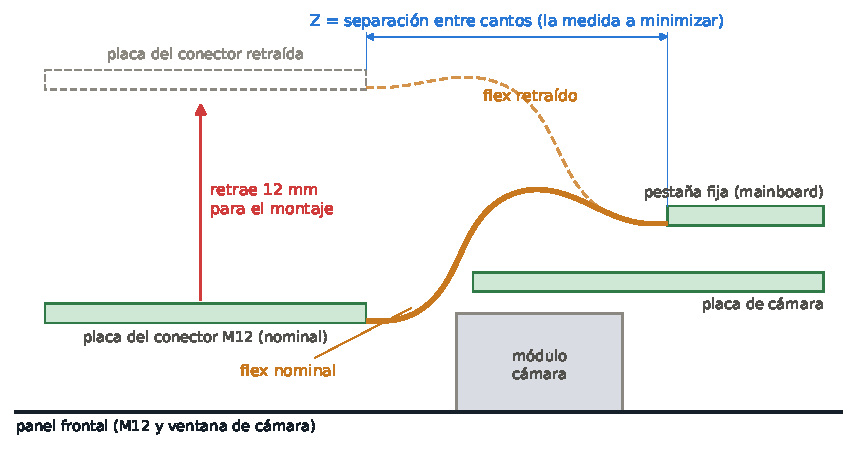
\includegraphics[width=0.98\linewidth]{assets/flex-problema.pdf}}
\caption*{\footnotesize\raggedright Figura 1 — Planta del conjunto como en Solid Edge, con el panel abajo. La placa del conector retrocede 12 mm y el flex pasa de la forma nominal (línea llena) a la retraída (línea de trazos). {\color{gray2}Esquema del autor sobre el layout del 27/9. Escala aproximada.}}
\end{figure}

\subsection*{1.2 Condiciones de diseño}
\addcontentsline{toc}{subsection}{1.2 Condiciones de diseño}

\begingroup\footnotesize
\setlength{\tabcolsep}{4pt}
\setlength{\emergencystretch}{4em}
\hyphenpenalty=50 \exhyphenpenalty=50
\begin{longtable}{@{}>{\RaggedRight\arraybackslash}p{\dimexpr 0.2634\linewidth-2\tabcolsep\relax}>{\RaggedRight\arraybackslash}p{\dimexpr 0.2926\linewidth-2\tabcolsep\relax}>{\RaggedRight\arraybackslash}p{\dimexpr 0.4390\linewidth-2\tabcolsep\relax}@{}}
\toprule
\scriptsize\textbf{Condición} & \scriptsize\textbf{Valor} & \scriptsize\textbf{De dónde sale} \\
\midrule
\endfirsthead
\toprule
\scriptsize\textbf{Condición} & \scriptsize\textbf{Valor} & \scriptsize\textbf{De dónde sale} \\
\midrule
\endhead
\bottomrule
\endfoot
Flex & 0,2 mm, 2 capas, 11 mm de alto & Lleva 48 V / 10 A y Ethernet \\
Radio interior mínimo & \textbf{2,5 mm} & 12 $\times$ espesor (IPC-2223, 2 capas, curva que se mueve pocas veces) \\
Recto en cada transición rígido-flex & 1 mm & Regla de fabricación \\
Carrera de la placa del conector & 12 mm (se verifica con 12,5) & Montaje a través del panel \\
Altura disponible en nominal & 12 $-$ 0,1 = 11,9 mm & Con cinta de 0,25 mm \\
Envolvente lateral & 52 mm, compartida con la cámara y el LED & Mecánica del equipo \\
Cantidad de flex & \textbf{uno solo} & Límite del fabricante (PCBWay) \\
Qué se minimiza & \textbf{Z}, la separación entre cantos & No el largo del flex \\
\end{longtable}
\endgroup

La cámara (e-con e-CAM52A, MIPI de 2 lanes) va apoyada en el piso, con el lente centrado en los 52 mm y su propio flex recto. En la vista de planta, su placa queda al lado de la S, 2,5 mm por detrás de la línea del flex del conector. Ese es el obstáculo que la S no puede tocar.

\clearpage

\section*{2. Método}
\addcontentsline{toc}{section}{2. Método}

Cada forma del flex se calculó y no se supuso. El flex se modela como una \textbf{elástica}: una tira inextensible con los dos extremos empotrados, que adopta la forma de mínima energía de flexión. Las paredes y la placa de cámara entran al modelo como obstáculos. Cada forma se resuelve en milisegundos, así que se puede recorrer toda la carrera y todas las combinaciones de tolerancias.

\begin{tarjeta}{Toda la carrera, ida y vuelta}{nominal $\rightarrow$ retraído $\rightarrow$ nominal}
Se barre la carrera en los dos sentidos, arrancando desde la posición nominal. Así aparece cualquier salto de forma que un barrido en un solo sentido esconde.

\end{tarjeta}
\begin{tarjeta}{Peor caso con tolerancias}{12 combinaciones por largo}
Cuerpo del conector de 6,3 a 7 mm ($\pm$ 0,35), carrera de 12 y 12,5 mm, largo del flex $\pm$ 0,25. Se informa siempre el peor resultado.

\end{tarjeta}
\begin{tarjeta}{Criterios de aceptación}{por forma}
R interior $\geq$ 2,5 en todo el recorrido y juego $\geq$ 0,3 a la placa de cámara, en nominal y durante toda la carrera.

\end{tarjeta}
\begin{notariesgo}{Lo que enseñó la simulación}
\textbf{Salto de forma (snap-through).} Cuando la S apoya contra una pared, en algún punto de la carrera salta de golpe a otra forma y el radio cae de repente. Esto no aparecía barriendo la carrera en un solo sentido. Por eso la S tiene que quedar \textbf{libre}, sin apoyar en nada, y centrada desde su propia pestaña.

\textbf{Largo mínimo.} Por debajo de un largo crítico el flex se tensa y se quiebra. Con este layout, eso ocurre bajo 18,5 mm (figura 5). El largo nominal se eligió lejos de ese borde, no pegado a él.

\end{notariesgo}
\clearpage

\section*{3. Cómo llegamos acá}
\addcontentsline{toc}{section}{3. Cómo llegamos acá}

Cada paso respondió a una limitación del anterior. W es el ancho total que ocupa la solución en el sentido de la carrera. Z es la separación entre cantos de la S.

\begingroup\footnotesize
\setlength{\tabcolsep}{4pt}
\setlength{\emergencystretch}{4em}
\hyphenpenalty=50 \exhyphenpenalty=50
\begin{longtable}{@{}>{\RaggedRight\arraybackslash}p{\dimexpr 0.0535\linewidth-2\tabcolsep\relax}>{\RaggedRight\arraybackslash}p{\dimexpr 0.3210\linewidth-2\tabcolsep\relax}>{\RaggedRight\arraybackslash}p{\dimexpr 0.2996\linewidth-2\tabcolsep\relax}>{\RaggedRight\arraybackslash}p{\dimexpr 0.3210\linewidth-2\tabcolsep\relax}@{}}
\toprule
\scriptsize\textbf{\#} & \scriptsize\textbf{Propuesta} & \scriptsize\textbf{Resultado} & \scriptsize\textbf{Qué se decidió} \\
\midrule
\endfirsthead
\toprule
\scriptsize\textbf{\#} & \scriptsize\textbf{Propuesta} & \scriptsize\textbf{Resultado} & \scriptsize\textbf{Qué se decidió} \\
\midrule
\endhead
\bottomrule
\endfoot
1 & Omega libre en el plano vertical, con la placa del conector colgando (9,5 $-$ R) & W $\approx$ 31–32 mm; con R 3 no entra en la altura & Buscar algo más angosto \\
2 & Omega del primer boceto & W = 26,4 mm, R 2,7 & Admitir R 2,5 (12 $\times$ espesor): W = 25,7 mm \\
3 & Placa del conector en el piso, flex hacia arriba & W $\approx$ 23–24 mm & Sigue ancho: pensar el flex en 3D \\
4 & \textbf{S de canto, en el plano de las placas} & W $\approx$ 13 mm & \textbf{Camino elegido} \\
5 & U rodante & Pide un canal libre de 7,6 mm & Descartada \\
6 & Integrar la cámara: imagen horizontal & Dobla demasiado el flex de la cámara & Cámara centrada con el flex recto (imagen a 90\textdegree{}) y pared lateral \\
7 & Cámara + S doble, islas de flex & Dos brazos de flex en una pieza & No fabricable: \textbf{un solo flex} \\
8 & LED junto al lente, sin guía de luz & Tres variantes (A, B, C) & Placa LED con conector B2B delante del flex de cámara \\
9 & Dimensionar la S & Z 15,5 con R 3, luego Z 14 con R 2,5; pestaña 5 mm atrás & Base del layout final \\
10 & \textbf{Layout del 27/9}, con la placa de cámara como obstáculo & Z = 15,5; L = 19,0 $\pm$ 0,25 & \textbf{Solución de este informe} \\
\end{longtable}
\endgroup

La galería de la sección 7 muestra cada alternativa en una imagen.

\clearpage

\section*{4. La solución}
\addcontentsline{toc}{section}{4. La solución}

La S sale del canto de la pestaña fija, retrocede un poco alejándose del panel, cruza por detrás de la placa de cámara y baja hasta la línea del flex en la placa del conector. En los dos extremos el flex sale por la cara delantera de la placa, con 1 mm recto antes de empezar a doblar.

Coordenadas usadas en todo el informe:

\begin{itemize}
\item \textbf{z}: hacia la derecha, desde el extremo izquierdo de la placa del conector.
\item \textbf{x}: hacia el panel, desde la línea del flex en la placa del conector (x = 0). Los valores negativos quedan detrás de esa línea.
\end{itemize}

\begingroup\footnotesize
\setlength{\tabcolsep}{4pt}
\setlength{\emergencystretch}{4em}
\hyphenpenalty=50 \exhyphenpenalty=50
\begin{longtable}{@{}>{\RaggedRight\arraybackslash}p{\dimexpr 0.6454\linewidth-2\tabcolsep\relax}>{\RaggedRight\arraybackslash}p{\dimexpr 0.1748\linewidth-2\tabcolsep\relax}>{\RaggedRight\arraybackslash}p{\dimexpr 0.1748\linewidth-2\tabcolsep\relax}@{}}
\toprule
\scriptsize\textbf{Referencia (nominal)} & \scriptsize\textbf{z} & \scriptsize\textbf{x} \\
\midrule
\endfirsthead
\toprule
\scriptsize\textbf{Referencia (nominal)} & \scriptsize\textbf{z} & \scriptsize\textbf{x} \\
\midrule
\endhead
\bottomrule
\endfoot
Canto de la placa del conector (salida del flex) & 16,50 & 0,00 \\
Canto de la pestaña fija (salida del flex) & 32,00 & $-$5,00 \\
Cara trasera de la placa de cámara & desde 22,0 & $-$2,50 \\
Inicio del módulo de cámara & 21,16 & — \\
\end{longtable}
\endgroup


\subsection*{4.1 Geometría para dibujar}
\addcontentsline{toc}{subsection}{4.1 Geometría para dibujar}

La forma real tiene radios variables. Para el modelo 3D no hace falta copiarla: alcanza con un perfil de \textbf{tres arcos del mismo radio, R 3,5, unidos por rectas}, con el mismo largo desarrollado y los mismos extremos y tangentes. En el equipo el flex va a tomar su forma natural, que es la simulada. El dibujo sirve para reservar el espacio y para obtener el largo desarrollado.

\begin{figure}[htbp]\centering
\fbox{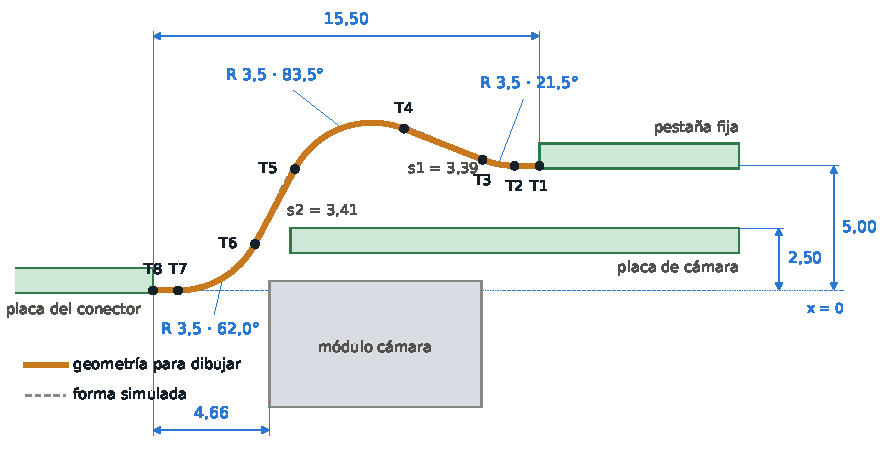
\includegraphics[width=0.98\linewidth]{assets/flex-geometria.pdf}}
\caption*{\footnotesize\raggedright Figura 2 — Perfil para dibujar, en posición nominal. La línea de trazos gris es la forma simulada; en ningún punto se aparta más de 0,11 mm del perfil de dibujo. Radios medidos en la línea media del flex. {\color{gray2}Elaboración propia. geom\_simple.py y s\_layout.py.}}
\end{figure}
Recorrido desde la pestaña fija (T1) hasta la placa del conector (T8):

\begingroup\footnotesize
\setlength{\tabcolsep}{3pt}
\setlength{\emergencystretch}{4em}
\hyphenpenalty=50 \exhyphenpenalty=50
\begin{longtable}{@{}>{\RaggedRight\arraybackslash}p{\dimexpr 0.0984\linewidth-2\tabcolsep\relax}>{\RaggedRight\arraybackslash}p{\dimexpr 0.1575\linewidth-2\tabcolsep\relax}>{\RaggedRight\arraybackslash}p{\dimexpr 0.1181\linewidth-2\tabcolsep\relax}>{\RaggedRight\arraybackslash}p{\dimexpr 0.2120\linewidth-2\tabcolsep\relax}>{\RaggedRight\arraybackslash}p{\dimexpr 0.1840\linewidth-2\tabcolsep\relax}>{\RaggedRight\arraybackslash}p{\dimexpr 0.2249\linewidth-2\tabcolsep\relax}@{}}
\toprule
\scriptsize\textbf{Tramo} & \scriptsize\textbf{Elemento} & \scriptsize\textbf{Medida} & \scriptsize\textbf{Gira hacia} & \scriptsize\textbf{Punto final (z; x)} & \scriptsize\textbf{Centro del arco (z; x)} \\
\midrule
\endfirsthead
\toprule
\scriptsize\textbf{Tramo} & \scriptsize\textbf{Elemento} & \scriptsize\textbf{Medida} & \scriptsize\textbf{Gira hacia} & \scriptsize\textbf{Punto final (z; x)} & \scriptsize\textbf{Centro del arco (z; x)} \\
\midrule
\endhead
\bottomrule
\endfoot
T1–T2 & Recta & 1,00 & — & 31,000; $-$5,000 & — \\
T2–T3 & Arco & R 3,5 \textperiodcentered{} 21,5\textdegree{} & atrás (se aleja del panel) & 29,717; $-$5,244 & 31,000; $-$8,500 \\
T3–T4 & Recta & 3,39 & — & 26,566; $-$6,485 & — \\
T4–T5 & Arco & R 3,5 \textperiodcentered{} 83,5\textdegree{} & adelante (hacia el panel) & 22,193; $-$4,871 & 25,284; $-$3,228 \\
T5–T6 & Recta & 3,41 & — & 20,590; $-$1,857 & — \\
T6–T7 & Arco & R 3,5 \textperiodcentered{} 62,0\textdegree{} & atrás, hasta quedar paralelo & 17,500; 0,000 & 17,500; $-$3,500 \\
T7–T8 & Recta & 1,00 & — & 16,500; 0,000 & — \\
 & \textbf{Total} & \textbf{19,00} &  &  &  \\
\end{longtable}
\endgroup

\begin{notadato}{Cómo trazarlo en Solid Edge}
\begin{enumerate}
\item Dibujar el croquis como una cadena de rectas y arcos tangentes.
\item Fijar los dos extremos: T1 en (32; $-$5) y T8 en (16,5; 0). En los dos, el flex sale paralelo a la placa.
\item Acotar los tres radios en \textbf{3,5} y las rectas de los extremos en \textbf{1,00}.
\item Acotar dos ángulos: \textbf{21,5\textdegree{}} y \textbf{62\textdegree{}}. El arco central queda determinado, porque 21,5 + 62 = 83,5\textdegree{} y así el flex llega paralelo a la placa del conector.
\item Las dos rectas intermedias (3,39 y 3,41) salen solas al cerrar el croquis.
\item Crear una \textbf{pestaña por contorno} sobre ese croquis: espesor 0,2, alto 11, factor neutro 0,5. El largo desarrollado da 19,00.
\end{enumerate}

\end{notadato}
Chequeos del perfil de dibujo: largo 19,002 mm; juego a la placa de cámara 1,93 mm. El radio interior de dibujo es 3,4 mm y el real es menor, 2,84 mm como mínimo. Por eso el radio se verifica siempre con la simulación, nunca con el dibujo.


\subsection*{4.2 Especificación para fabricar}
\addcontentsline{toc}{subsection}{4.2 Especificación para fabricar}

\begingroup\footnotesize
\setlength{\tabcolsep}{4pt}
\setlength{\emergencystretch}{4em}
\hyphenpenalty=50 \exhyphenpenalty=50
\begin{longtable}{@{}>{\RaggedRight\arraybackslash}p{\dimexpr 0.3666\linewidth-2\tabcolsep\relax}>{\RaggedRight\arraybackslash}p{\dimexpr 0.6284\linewidth-2\tabcolsep\relax}@{}}
\toprule
\scriptsize\textbf{Parámetro} & \scriptsize\textbf{Valor} \\
\midrule
\endfirsthead
\toprule
\scriptsize\textbf{Parámetro} & \scriptsize\textbf{Valor} \\
\midrule
\endhead
\bottomrule
\endfoot
Largo del flex entre cantos rígidos & \textbf{19,0 $\pm$ 0,25 mm} \\
Largo mínimo absoluto & 18,5 mm: por debajo, el flex se tensa y apoya en la placa de cámara \\
Rectos en las transiciones & 1,0 mm en cada extremo, sin cobre cruzando la línea de doblez \\
Espesor y capas & 0,2 mm, 2 capas \\
Alto del flex & 11 mm \\
Separación entre cantos (Z) & 15,5 mm \\
Salida del flex & Cara delantera de las dos placas \\
\end{longtable}
\endgroup

\begin{detalle}{Perfil exacto de la forma simulada (referencia, desvío 0,02 mm)}
Es el ajuste por arcos de la forma de equilibrio en nominal, el mismo que figura en el plano FX-M12-S-03 y en el DXF \texttt{S\_conector\_layout27\_nominal.dxf}. No hace falta para dibujar; queda como registro.

\begingroup\footnotesize
\setlength{\tabcolsep}{4pt}
\setlength{\emergencystretch}{4em}
\hyphenpenalty=50 \exhyphenpenalty=50
\begin{longtable}{@{}>{\RaggedRight\arraybackslash}p{\dimexpr 0.1216\linewidth-2\tabcolsep\relax}>{\RaggedRight\arraybackslash}p{\dimexpr 0.3479\linewidth-2\tabcolsep\relax}>{\RaggedRight\arraybackslash}p{\dimexpr 0.2214\linewidth-2\tabcolsep\relax}>{\RaggedRight\arraybackslash}p{\dimexpr 0.3041\linewidth-2\tabcolsep\relax}@{}}
\toprule
\scriptsize\textbf{\#} & \scriptsize\textbf{Elemento} & \scriptsize\textbf{Desde (z; x)} & \scriptsize\textbf{Medida} \\
\midrule
\endfirsthead
\toprule
\scriptsize\textbf{\#} & \scriptsize\textbf{Elemento} & \scriptsize\textbf{Desde (z; x)} & \scriptsize\textbf{Medida} \\
\midrule
\endhead
\bottomrule
\endfoot
1 & Recta & 32,000; $-$5,000 & 1,000 \\
2 & Arco antihorario & 31,000; $-$5,000 & R 3,677 \textperiodcentered{} 23,2\textdegree{} \\
3 & Recta & 29,549; $-$5,298 & 2,890 \\
4 & Arco horario & 26,893; $-$6,439 & R 3,828 \textperiodcentered{} 86,6\textdegree{} \\
5 & Recta & 21,960; $-$4,635 & 2,659 \\
6 & Arco antihorario & 20,769; $-$2,258 & R 4,376 \textperiodcentered{} 35,7\textdegree{} \\
7 & Arco antihorario & 18,890; $-$0,342 & R 2,990 \textperiodcentered{} 27,7\textdegree{} \\
8 & Recta & 17,500; 0,000 & 1,000 hasta 16,500; 0,000 \\
\end{longtable}
\endgroup

\end{detalle}
\clearpage

\section*{5. Verificación en toda la carrera}
\addcontentsline{toc}{section}{5. Verificación en toda la carrera}

\begin{figure}[htbp]\centering
\fbox{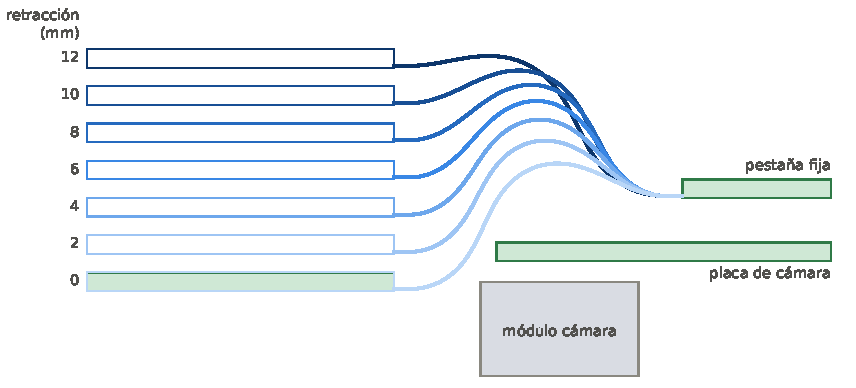
\includegraphics[width=0.98\linewidth]{assets/flex-carrera.pdf}}
\caption*{\footnotesize\raggedright Figura 3 — Forma del flex cada 2 mm de retracción, de 0 (nominal) a 12 mm. La S se abre hacia atrás y nunca toca la placa de cámara. {\color{gray2}Simulación de la elástica. s\_layout.py.}}
\end{figure}
\begin{figure}[htbp]\centering
\fbox{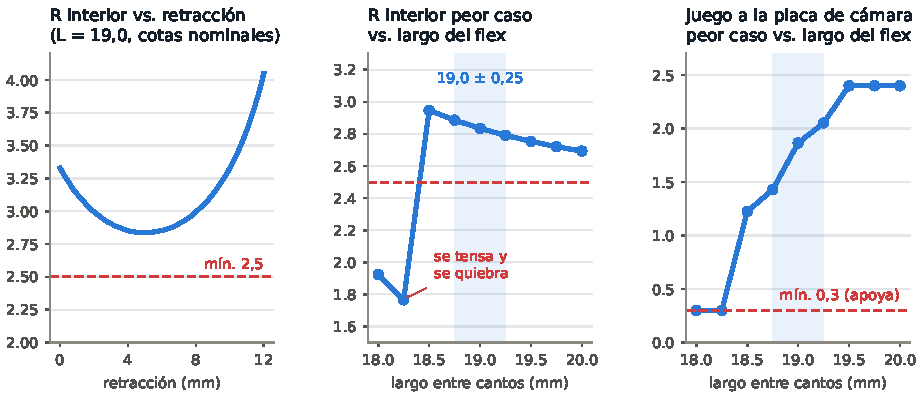
\includegraphics[width=0.98\linewidth]{assets/flex-robustez.pdf}}
\caption*{\footnotesize\raggedright Figura 4 y 5 — Izquierda: R interior a lo largo de la carrera, con L = 19,0 y cotas nominales; el mínimo es 2,84 mm, cerca de los 5 mm de retracción. Centro y derecha: peor caso de R interior y de juego a la placa de cámara según el largo del flex. La banda marca 19,0 $\pm$ 0,25. {\color{gray2}Simulación de la elástica. Peor caso sobre el cuerpo del conector de 6,3 a 7 mm y la carrera de 12 y 12,5 mm.}}
\end{figure}
\begingroup\footnotesize
\setlength{\tabcolsep}{4pt}
\setlength{\emergencystretch}{4em}
\hyphenpenalty=50 \exhyphenpenalty=50
\begin{longtable}{@{}>{\RaggedRight\arraybackslash}p{\dimexpr 0.1841\linewidth-2\tabcolsep\relax}>{\RaggedRight\arraybackslash}p{\dimexpr 0.2630\linewidth-2\tabcolsep\relax}>{\RaggedRight\arraybackslash}p{\dimexpr 0.1972\linewidth-2\tabcolsep\relax}>{\RaggedRight\arraybackslash}p{\dimexpr 0.3507\linewidth-2\tabcolsep\relax}@{}}
\toprule
\scriptsize\textbf{Largo del flex} & \scriptsize\textbf{R interior peor caso} & \scriptsize\textbf{Juego peor caso} & \scriptsize\textbf{Veredicto} \\
\midrule
\endfirsthead
\toprule
\scriptsize\textbf{Largo del flex} & \scriptsize\textbf{R interior peor caso} & \scriptsize\textbf{Juego peor caso} & \scriptsize\textbf{Veredicto} \\
\midrule
\endhead
\bottomrule
\endfoot
18,25 & 1,77 & 0,30 & No: se tensa y apoya \\
18,50 & 2,95 & 1,22 & Borde: sin margen para la tolerancia \\
\textbf{18,75} & \textbf{2,89} & \textbf{1,43} & Sí (tolerancia $-$) \\
\textbf{19,00} & \textbf{2,84} & \textbf{1,87} & \textbf{Sí (nominal)} \\
\textbf{19,25} & \textbf{2,79} & \textbf{2,05} & Sí (tolerancia +) \\
20,00 & 2,69 & 2,40 & Sí, pero ocupa más \\
\end{longtable}
\endgroup

Dentro de la tolerancia de fabricación, el peor caso es \textbf{R interior 2,79 mm} con L = 19,25 y \textbf{juego 1,43 mm} con L = 18,75. Los dos cumplen con margen.

\clearpage

\section*{6. Supuestos y puntos abiertos}
\addcontentsline{toc}{section}{6. Supuestos y puntos abiertos}

\begin{notainferencia}{Supuestos de lectura del layout del 27/9}
\begin{itemize}
\item La cota \textbf{2,5} es la distancia desde la cara trasera de la placa de cámara hasta la línea del flex en la placa del conector, medida hacia atrás.
\item La placa de cámara empieza en z $\approx$ 22 y el módulo, 4,66 mm después del canto de la placa del conector.
\item Juego mínimo exigido al flex: 0,3 mm.
\item El flex se modela con rigidez uniforme. El cobre de las dos capas cambia la rigidez, pero no el largo ni la forma general.
\end{itemize}

Si alguna de estas cotas cambia, se vuelve a correr \texttt{s\_layout.py} y se regeneran el plano y este informe.

\end{notainferencia}
Queda por confirmar con una muestra: el largo real entre cantos después del fresado del rígido, y el comportamiento del flex con el cobre en el ciclo de montaje.

\clearpage

\section*{7. Alternativas evaluadas}
\addcontentsline{toc}{section}{7. Alternativas evaluadas}

Cada imagen es una de las propuestas que se simularon o modelaron en el camino. El resultado de cada una está en una línea; la marca verde indica que la idea sobrevivió, total o parcialmente, en la solución final.

\begin{figure}[htbp]\centering
\fbox{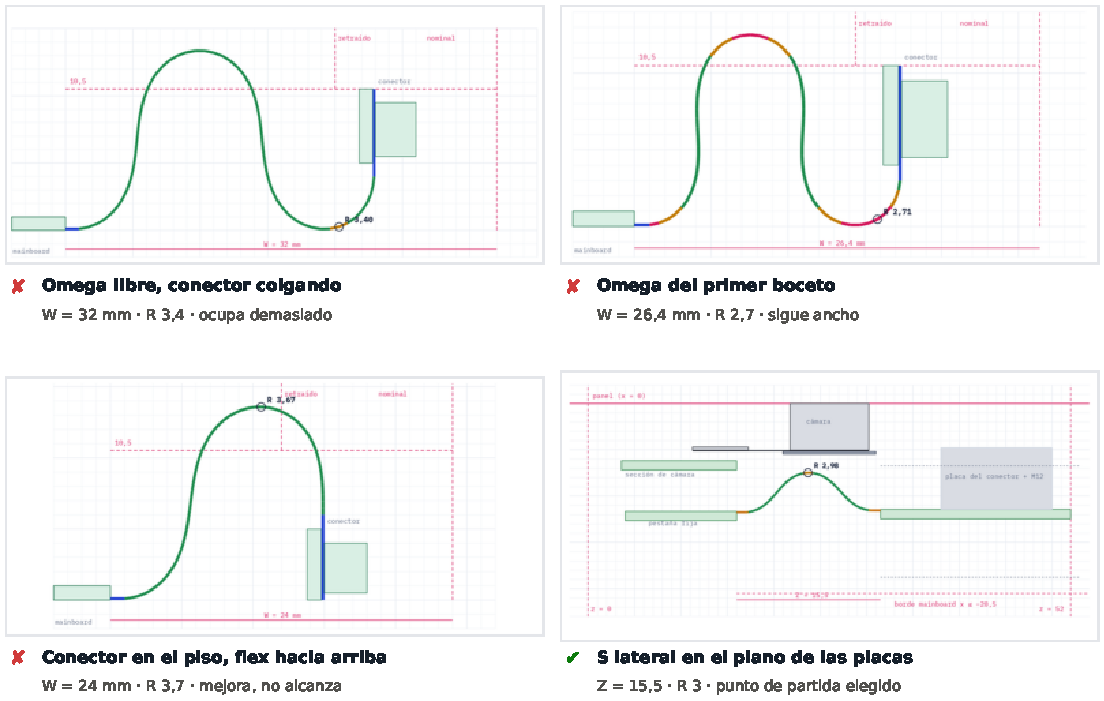
\includegraphics[width=0.98\linewidth]{assets/flex-galeria-1.pdf}}
\caption*{\footnotesize\raggedright Figura 6 — Primer grupo: formas en el plano vertical (omega) y la primera S en el plano de las placas. {\color{gray2}Capturas de las páginas de simulación 2D.}}
\end{figure}
\begin{figure}[htbp]\centering
\fbox{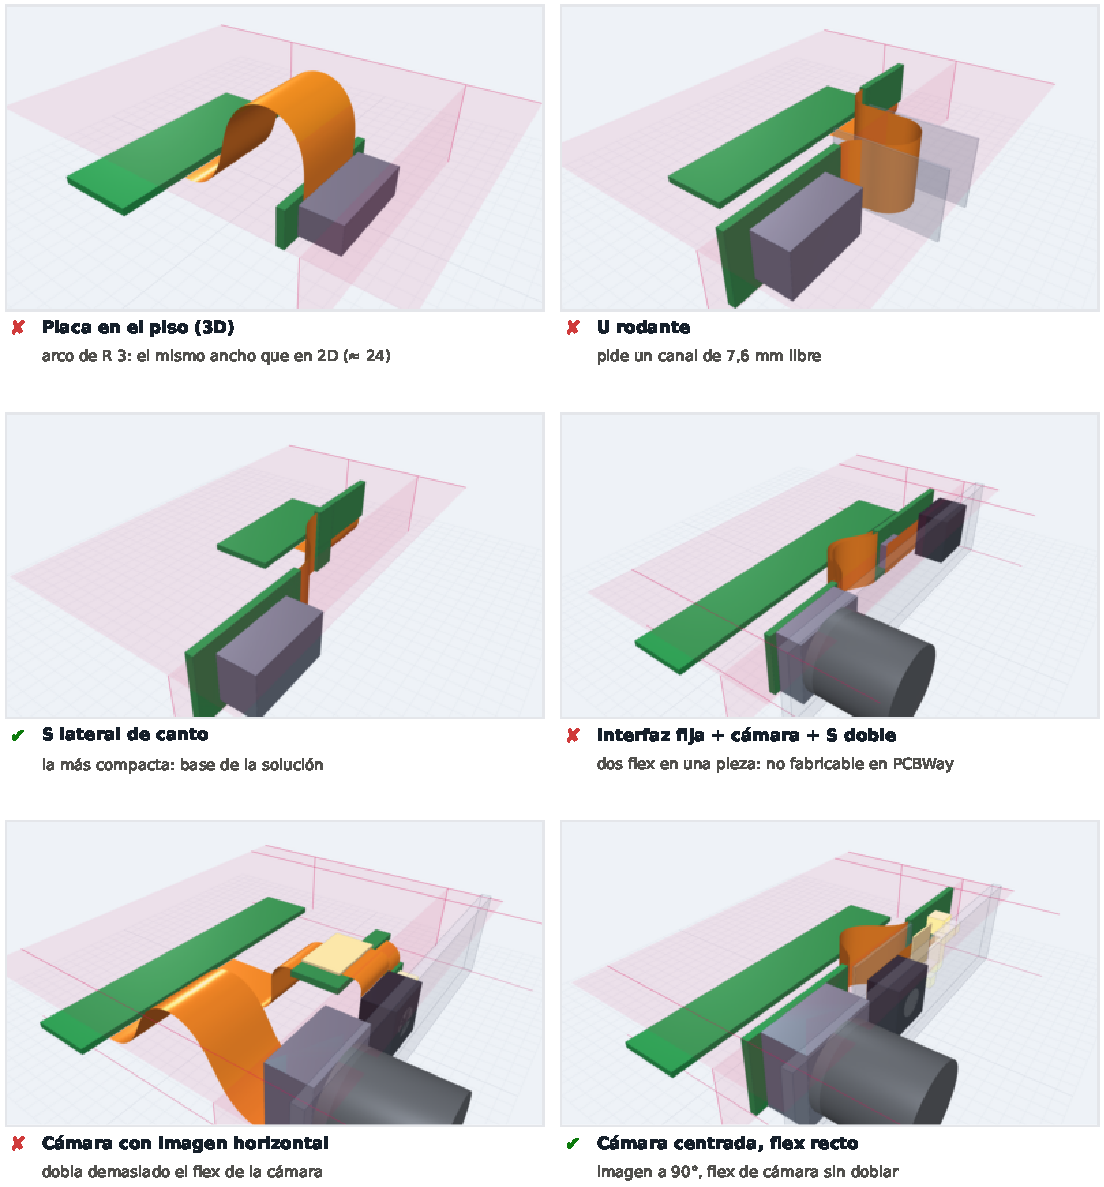
\includegraphics[width=0.98\linewidth]{assets/flex-galeria-2.pdf}}
\caption*{\footnotesize\raggedright Figura 7 — Segundo grupo: arquitecturas en 3D e integración de la cámara. {\color{gray2}Capturas del visor 3D de opciones.}}
\end{figure}
\begin{figure}[htbp]\centering
\fbox{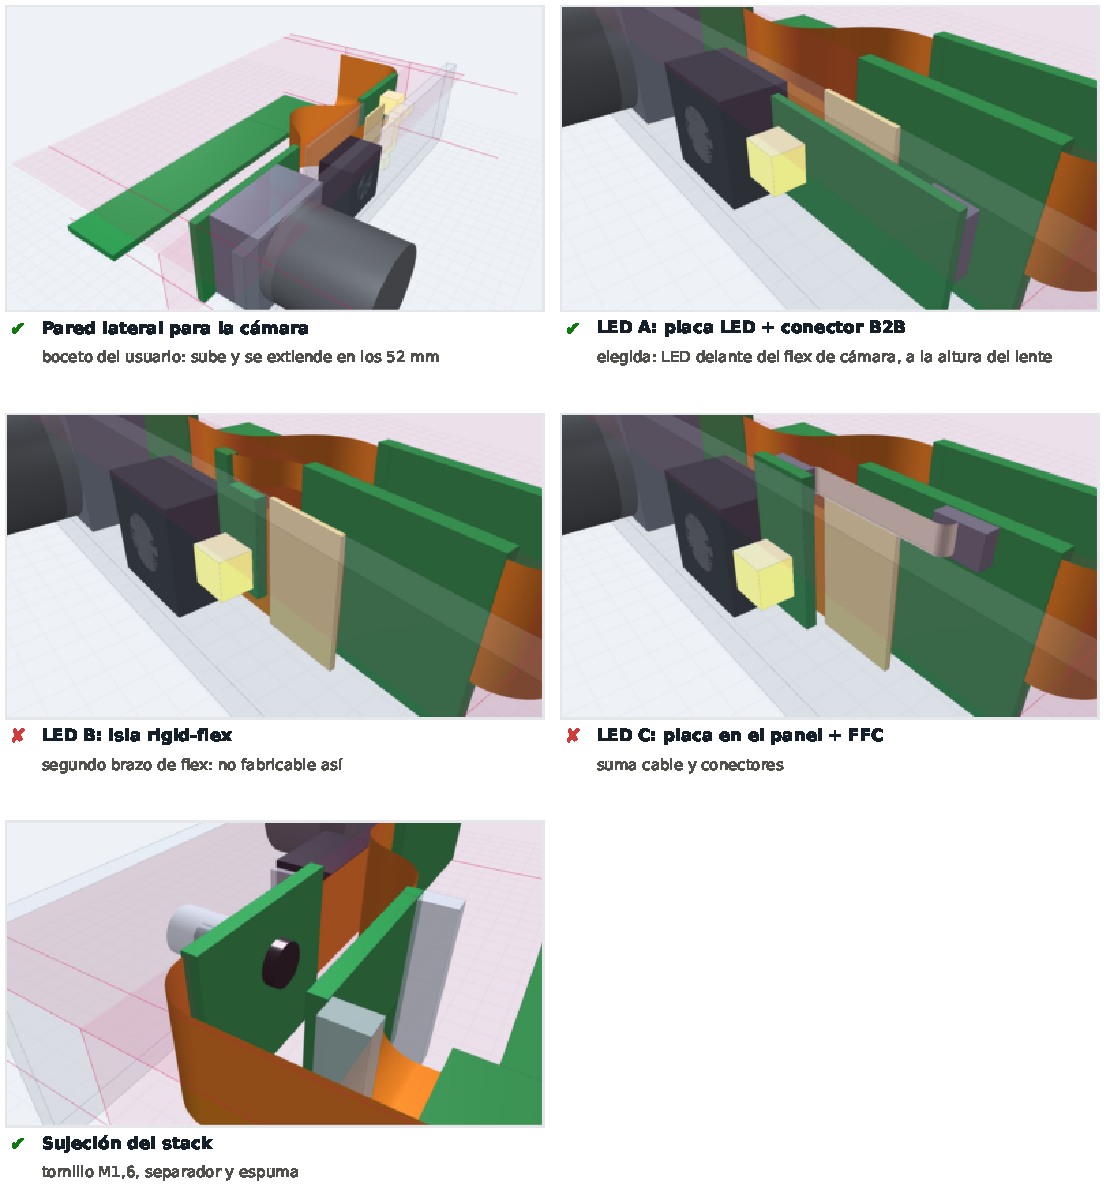
\includegraphics[width=0.98\linewidth]{assets/flex-galeria-3.pdf}}
\caption*{\footnotesize\raggedright Figura 8 — Tercer grupo: cámara en la pared lateral y variantes del LED. {\color{gray2}Capturas del visor 3D de opciones.}}
\end{figure}
\clearpage

\section*{Anexo — Archivos}
\addcontentsline{toc}{section}{Anexo — Archivos}

\begingroup\footnotesize
\setlength{\tabcolsep}{4pt}
\setlength{\emergencystretch}{4em}
\hyphenpenalty=50 \exhyphenpenalty=50
\begin{longtable}{@{}>{\RaggedRight\arraybackslash}p{\dimexpr 0.4856\linewidth-2\tabcolsep\relax}>{\RaggedRight\arraybackslash}p{\dimexpr 0.5094\linewidth-2\tabcolsep\relax}@{}}
\toprule
\scriptsize\textbf{Archivo (en \texttt{flex\_omega\slash })} & \scriptsize\textbf{Qué contiene} \\
\midrule
\endfirsthead
\toprule
\scriptsize\textbf{Archivo (en \texttt{flex\_omega\slash })} & \scriptsize\textbf{Qué contiene} \\
\midrule
\endhead
\bottomrule
\endfoot
\texttt{s\_layout.py} $\rightarrow$ \texttt{s\_layout.json} & Modelo final: forma nominal, carrera, peor caso por largo y perfil ajustado \\
\texttt{plano\_layout.py} $\rightarrow$ plano PDF en \texttt{planos/} & Plano FX-M12-S-03: planta 4:1, desarrollo de la tira, tangencias \\
\texttt{planos/\dots{}nominal.dxf} & Perfil exacto en nominal, para importar en Solid Edge \\
\texttt{informe/geom\_simple.py} $\rightarrow$ \texttt{geom\_simple.json} & Geometría para dibujar: tres arcos R 3,5 \\
\texttt{informe/figuras.py} & Figuras de este informe \\
\texttt{s\_layout.html} & Animación 2D de la carrera con el layout final \\
\texttt{opciones3d.html} & Visor 3D de todas las alternativas \\
\end{longtable}
\endgroup


\end{document}
